Основным элементом задетекторной считывающей электроники жидкоаргонового калориметра детектора ATLAS в рамках второй фазы обновления являются модули сигнального процессора LASP (Liquid Argon Signal Processor). Они предназначены для принятия оцифрованных данных с модулей FEB2 и применения к ним цифровой фильтрации, их буферизации до появления сигнала триггера и последующей передачи в систему сбора данных DAQ. Также система LASP обеспечивает подготовку входныз данных для таких систем, как глобальный триггер и fFEX(forward Feature EXtractor). Система глобального триггера будет получать значения энергий только от тех ячеек, которые превышают заданный порог, определённый относительно общего шума. Таким образом, полосой пропускания данных можно управлять, сохраняя при этом достаточную количество информации для кластеризации событий.\par
Сигнальные процессоры рассчитаны на приём непрерывного потока оцифрованных данных с плат FEB2 на частоте соударения пучков частиц в Большом Адронном коллайдере (фактическая частота составляет 40.07897 МГц) для всех 182486 ячеек жидкоаргонового калориметра. Каждый модуль будет получать исходные данные с 8 плат FEB2, то есть с 1024 калориметрических ячеек. В настоящее время ведётся активная разработка этой системы.\par
Модули LASP требуют высокой пропускной способности ввода и вывода, а также возможности гибкого программирования алгоритмов обработки данных, цифровой фильтрации и сокращения объёма данных, поэтому в качестве основных вычислительных блоков LASP предусмотрены программируемые интегральные микросхемы. На плате каждого модуля будет располагаться 2 таких чипа для увеличения пропускной способности. Внутренняя структура дизайна программируемой логики представлена на рисунке \ref{fig:lasp}.

\begin{figure}[ht]
    \centering
    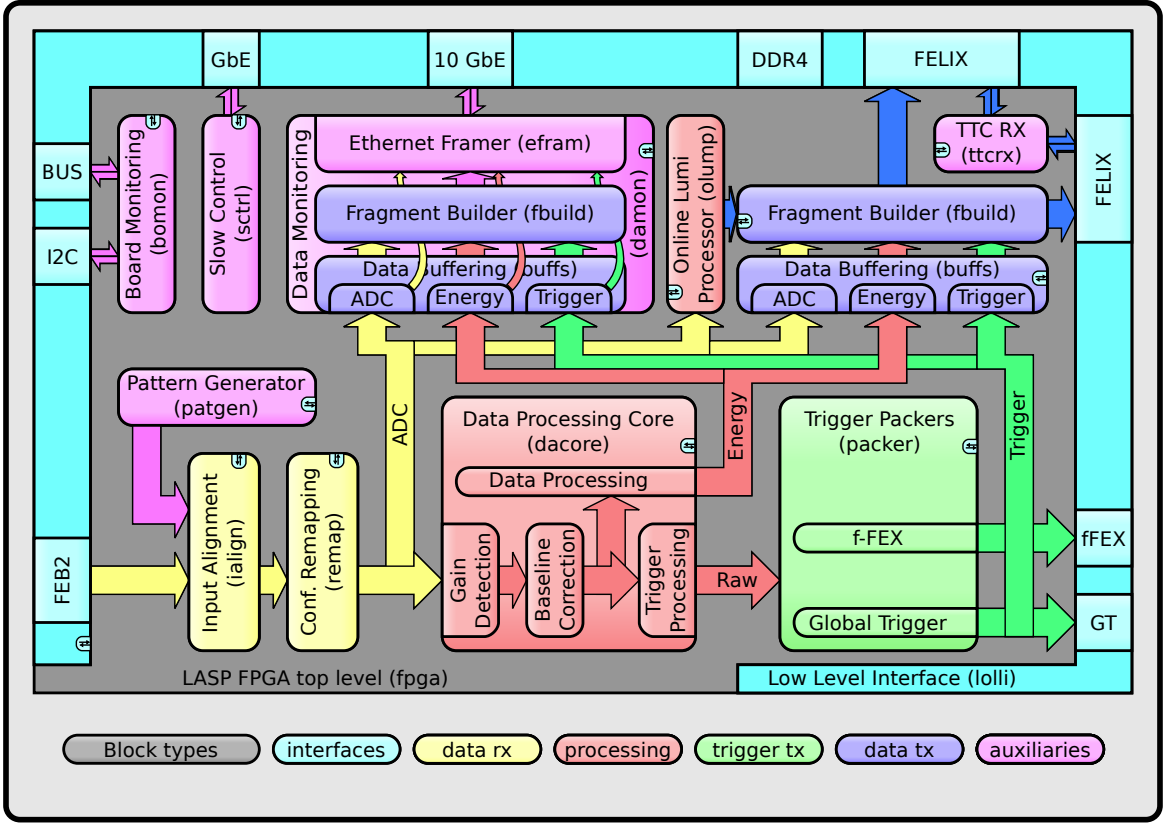
\includegraphics[width=\linewidth]{lasp.png}
    \caption{Блок схема архитектуры сигнального процессора LASP}
    \label{fig:lasp}
\end{figure}\par

Основными модулями сигнального процессора LASP являются:\par
\begin{itemize}
    \item интерфейс нижнего уровня lolli;
    \item система медленного контроля sctrl;
    \item генератор тестовых сигналов patgen;
    \item выравниватель входных данных ialign;
    \item модуль конфигурируемой перестановки remap;
    \item ядро обработки данных dacore;
    \item процессор онлайн светимости olump;
    \item упаковщик триггерных данных packer;
    \item блок буферов buffs;
    \item модуль форматирования данных fbuild;
    \item модуль мониторинга данных damon;
    \item монитор состояния аппаратуры bomon.
\end{itemize}\par

Для работы сигнального процессора используется целый набор различных тактовых сигналов. Среди основных можно выделить:
\begin{itemize}
    \item $f_{feb}$ -- тактовая частота, синхронно с которой поступают входные данные с системы FEB2. Имеет фиксированное значение 320 МГц;
    \item $f_{core}$ --  тактовая частота, синхронно с которой происходит непосредственная обработка данных. В зависимости от конфигурации может быть либо 320 МГц -- так называемая медленная опция, либо 480 МГц -- быстрая опция;
    \item $f_{sctrl}$ -- тактовая частота, на которой функционирует интерфейс медленного контроля. Непосредственное значение составляет 100 МГц.
    \item $f_{xgbe}$ -- тактовая частота, необходимая для приёма и отправки данных через 10 Гбит Ethernet порт(X Gigabit Ethernet). Является стендартной для такого порта и составляет 156,25 МГц.
\end{itemize}\par
\textbf{Интерфейс нижнего уровня lolli}\par
Также в системе присутствует ещё несколько вспомогательных тактовых сигналов, необходимых для работы DDR4 интерфейса и TTC RX.\par
Базовым модулем системы LASP, с помощью которого осуществляется взаимодействие с внешним миром, является интерфейс нижнего уровня lolli. Данная подсистема содержит реализации всех необходимых низкоуровневых внешних интерфейсов:\par
\begin{itemize}
    \item FEB2;
    \item Gigabit Ethernet;
    \item 10 Gigabit Ethernet;
    \item DDR4 SDRAM;
    \item I2C;
    \item Custom BUS;
    \item fFEX;
    \item FELIX;
    \item Global Trigger.
\end{itemize}\par
При возможности, все интерфейсы из lolli в программируемую логику спроектированы с использованием стандартных потокового интерфейса Avalon Stream (AVST) и интерфейса, отображаемого на память Avalon Memory Mapped (AVMM). Это позволяет иметь четко определённые и документированные стандартные интерфейсы между каждым компонентом LASP.\par
\textbf{Система медленного контроля sctrl}\par
Для реализации возможности управления всеми компонентами сигнального процессора, а также их соединения с внешним миром предусмотрена система медленного контроля sctrl. Она позволяет пользователю загружать или изменять все доступные пользователю параметры конфигурации, а также иметь доступ ко всем регистрам мониторинга и состояния любого модуля в режиме реального времени.\par
Компонент sctrl использует внешний канал связи Gigabit Ethernet, реализованный в интерфейсе lolli. Для общения с внутренними модулями используется AVMM интерфейс. Специально для интерфейса медленного контроля каждый модуль имеет набор выделенных регистров, в которых хранятся либо какие-нибудь параметры, либо данные о состоянии или некоторая статистика. Между этими регистрами есть глобальное разделение адресного пространства, через которое sctrl и способно доступаться к конкретным модулям.\par
\textbf{Генератор тестовых данных patgen}\par
В целях отладки системы в общей структуре релизован генератор тестовых данных patgen. С его помощью можно осуществлять ввод определяемых пользователем значений АЦП для обработки вместо данных, поступающих от FEB2. Такая возможность используется для тестирования системы и проверки основного функционала независимо от реальных данных с FEB2. Для корректной отладки с помощью pathen в него заложены следующие свойства:\par
\begin{itemize}
    \item данные, генерируемые patgen имеют ту же структуру, что и данные из FEB2;
    \item patgen способен иммитировать рассинхронизацию между каналами данных(сдвиг по идентификатору пучка);
    \item каждый канал имеет независмый источник данных;
    \item имеется возможность выбирать между двумя возможными источниками данных(patgen или FEB2) для каждого канала данных в отдельности;
    \item данные генерируются непрерывно циклическим образом, повторение происходит синхронизованно с циклом пучков на орбите.
\end{itemize}\par
Для снижения влияния на процесс компиляции системы целиком в проектирование генератор тестовых сигналов заложен принцип минимизации занимаемых логических ресурсов. В следствие этого, patgen имеет две версии реализации:\par
\begin{itemize}
    \item на основе оперативной памяти: в этой версии используются данные, хранимые во внутренней операвтивной памяти ПЛИС, записанные через интерфейс медленного контроля. Такой подход даёт большую гибкость, но занимает большой объём памяти;
    \item на основе функции генерации: в этой версии данные генерируются на лету, используя определённый алгоритм.
\end{itemize}\par
\textbf{Выравниватель входных данных ialign}\par
Первым модулем, который непосредственно принимает входные данные, является ialign. Он предназначен для осуществления выравнивания по времени поступающей информации с FEB2. Входной поток организован в виде кадров, содержащих данные АЦП и два идентификатора столкновения пучков для соответствующих шкал усиления, которые могут быть как идентичными, так и различными. В ходе обработки все данные АЦП выравниваются по одинаковому BCID. При этом порядок оцифрованных значений в рамках каждого отдельного канала может изменяться, однако он не предопределён заранее -- его можно настраивать индивидуально для любого потока, но идентично для парных значений по шкалам усиления.\par
Важная особенность обработки данных модулем ialign -- это расширение данных по временным ячейкам. То есть, по всем каналам с низкого уровня поступает по 6 значений АЦП для каждого идентификатора столкновения пучков, но данный модуль добавляет везде по 2 дополнительных невалидных значения, тем самым увеличивая число временных ячеек с данными АЦП до 8. На рисунке \ref{fig:ialign_output} схематично изображён выходной интерфейс компонента. Рабочей тактовой частотой для ialign является $f_{feb}$, соответствующая поступающим с FEB2 данным.

\begin{figure}[ht]
    \centering
    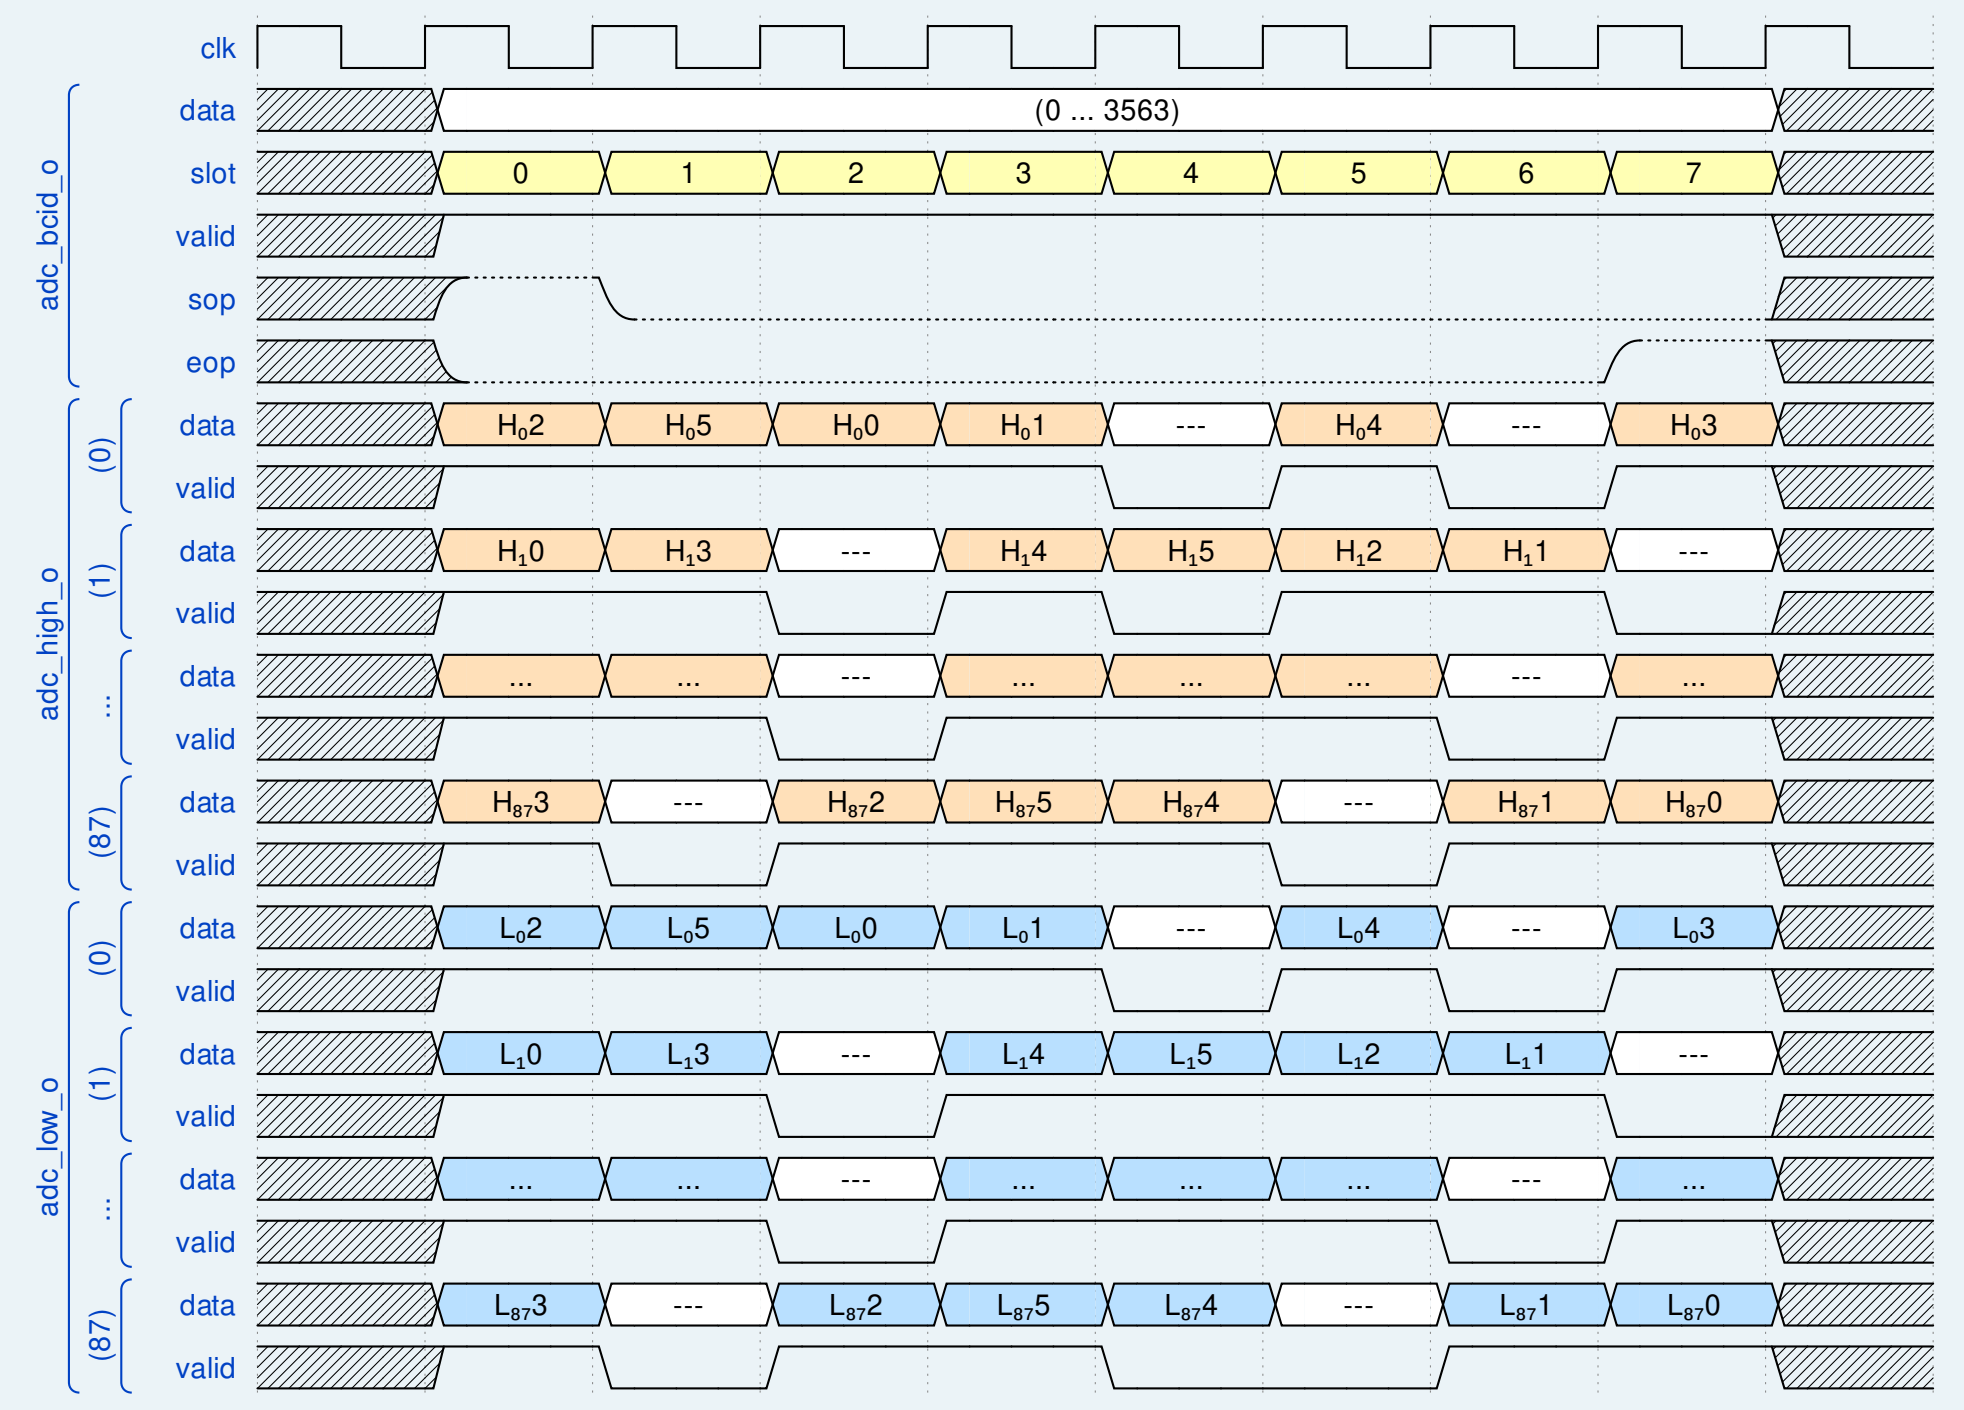
\includegraphics[width=\linewidth]{ialign_output.png}
    \caption{Выходной интерфейс модуля ialign}
    \label{fig:ialign_output}
\end{figure}\par

\textbf{Модуль конфигурируемой перестановки remap}\par
Следующий элемент тракта данных жидкоаргонового сигнального процессора LASP -- модуль remap. Он служит для изменения порядка данных в соответствии с геометрией детектора, ведь в силу ряда технических ограничений, информация от калориметрических ячеек, поступающая через FEB2, находится в перемешанном виде. Путём переупорядочивания данных упрощается задача вычисления сумм энергии ячеек жидкоаргонового калориметра. Такие суммы необходимы для уменьшения полосы пропускания данных в системе fFEX. Как и в случае модуля ialign схема перестановки не является предопределённой -- каждый выходной канал может быть гибко сконфигурирован согласно требованиям. Важной особенностью является то, что помимо всего прочего, компонент конфигурируемой перестановки необходим для реализации перехода данных из тактового домена $f_{feb}$ в домен сигнала $f_{core}$.\par
Сигнальный процессор LASP может иметь одну из двух конфигураций, так называемые медленную и быструю опции. В случае медленной опции remap принимает входной поток данных, состоящий из 88 каналов, в которых содержится по 8 значений АЦП для каждого идентификатора соударения пучка и преобразовывыет его в аналогичный поток, но имеющий лишь 64 точно таких же канала. При этом тактовые частоты $f_{feb}$ и $f_{core}$ совпадают по величине 320 МГц, однако могут быть сдвинутыми по фазе. Реальный объём полезных данных не уменьшается, как это может показаться на первый взгяд, поскольку четверть входного трафика составляют невалидные значения, добавленные модулем ialign, а также присутствуют сигналы, поступающие с неподключнных разъёмов FEB2. В конфигурации быстрой опции та же структура входных данных преобразовывается в 43 выходных канала, каждый из которых имеет целых 12 оцифрованных величин. Поскольку в любом варианте интервал между соседними моментами соударения пучков не изменяется и составляет 25 наносекунд, то в таком режиме тактовая частота выходной шины $f_{core}$ пропорционально увеличена и составляет 480 МГц для обеспечения необходимой плотности данных во времени.\par
\textbf{Ядро обработки данных dacore}\par
Основным обрабатывающим компонентом процессора LASP является ядро обработки данных dacore. Оно преобразовывает поступающие от модуля конфигурируемой перестановки исходные значения АЦП в соответствующие энергетические величины с помощью специальных алгоритмов. Задачи обработки можно разделить на четыре основных функции:\par
\begin{itemize}
    \item определение оптимального коэффициента усиления;
    \item коррекция пъедистала;
    \item вычисление энергии, временной характеристики, а также параметра качества с оптимальным разрешением для системы хранения данных (однако вычисление параметра качества и временной характеристики выполняется только для калориметрических ячеек с выделившейся в них энергией выше заданного порога);
    \item вычисление энергии с уменьшенным разрешением для триггерной системы.
\end{itemize}\par
Следовательно, компонент dacore обеспечивает 2 отдельных выходных потока:\par
\begin{enumerate}
    \item поток для модуля упаковки данных packer, который содержит грубые энергетические значения и флаги превышения порога;
    \item поток для блока буферов, содержащий для каждой калориметрической ячейки энергетическоt значениt, бит оптимального коэффициента усиления и флаг превышения порога. Для высокоэнергетических ячеек добавляется время импульса и значение качества импульса.
\end{enumerate}\par
Для повышения точности данных, направляемых в систему хранения, используется дополнительная стадия обработки, реализующая алгоритмы цифровой фильтрации. С их помощью достигается восстановление энергии с точностью 1 МэВ, которая затем кодируется многолинейным способом.Для триггерных данных также предусмотрена цифровая фильтрация, предназначенная для подавления шумов и вычисление значений энергии с достаточной точностью для всех модулей принятия триггерных решений, подключенных к задетекторной электронике. Также для этих данных формируется по три бита превышения порогов, количественно описывающие переполнения фонового уровня энергии.\par
\textbf{Процессор онлайн светимости olump}\par
Одним из важнейших показателей работы коллайдера является светимость. Для его рассчёта в системе жидкоаргонового сигнального процессора предусмотрен модуль процессора онлайн светимости olump. Этот компонент усредняет необработанные оцифрованные значения АЦП, получаемые напрямую с модуля конфигурируемой перестановки remap, по каждому столкновению частиц. Его задачи можно разделить на 4 основных части:\par
\begin{enumerate}
    \item вычисление суммы и суммы квадратов измерений АЦП по шкале высокого коэффициента усиления для настраиваемого набора из 8 каналов. Эти величины вычисляются для каждого столкновения пучков и накапливаются по каждому набору;
    \item буферизация данных АЦП по шкале высокого коэффициента усиления в течение одного полного оборота пучков на орбите Большого Адронного коллайдера. Производится это по тем же наборам каналов, которые были определены выше;
    \item вычисление оценки мгновенной светимости для этих же подмножеств каналов. Эта оценка может быть использована в ядре обработки данных dacore для компенсации влияния светимости на восстановление энергетических и временных величин;
    \item сжатие без потерь значений сумм и сумм квадратов оцифрованных сигналов АЦП.
\end{enumerate}\par
\textbf{Упаковщик триггерных данных packer}\par
Подготовка энергетических значений для их последующей передачи в триггерные системы задетекторной электроники осуществляется силами упаковщика триггерных данных packer. Задачи этого компонента заключаются в следующем:\par
\begin{itemize}
    \item группировка данных, полученных с ядра обработки данных;
    \item кодирование энергий с использованием многолинейного кодирования и их передача в системы глобального триггера и fFEX;
    \item отправка данных в блок буфферов;
    \item отправка данных в модуль damon.
\end{itemize}\par
Поток выходных данных для систем глобального триггера и fFEX состоит из кадров, которые содержат информацию о текущем соударении пучков. Помимо этого, в выходном канале требуется отправка служебных кадров, которые не содержат непосредственно полезные данные, а несут различную идентификационную информацию, необходимую, например, для синхронизации.\par
\textbf{Блок буферов buffs}\par
После обработки данные не сразу отправляются в систему хранения, а некоторое время ожидают соответствующего им триггерного сигнала в блоке буферов buffs. Буферизации подлежат все имеющиеся данные: изначальные значения АЦП, обработанные энергетические величины и триггерные данные, полученные от компонентов конфигурируемой перестановки remap, ядра обработки dacore и упаковщика packer соответственно. Время хранения информации требуется не меньшее, чем задержка триггера, которая составляет около 10 мкс.\par
\textbf{Модуль форматирования данных fbuild}\par
Последний этап обработки данных -- формирование из готовых значений фрагментов, пригодных к отправке в FELIX через интерфейс нижнего уровня lolli. Эта задача выполняется с помощью модуля форматирования данных fbuild. Генерируемый формат данных может варьироваться в зависимости от назначения:\par
\begin{itemize}
    \item сбор данных;
    \item калибровка;
    \item отладка;
    \item тестирование системы;
    \item ввод в эксплуатацию.
\end{itemize}\par
Данные, содержащиеся во фрагментах, представляют собой исходные данные АЦП или энергетические значения и связанные с ними биты валидности и качества, а также данные, отправляемые в системы глобального триггера и fFEX. Формат кадра может потребовать отправки определённых или всех этих типов данных. Кроме того, можно выбирать один или несколько потоков выходных данных, хотя обычно используются все.\par
\textbf{Модуль мониторинга данных damon}\par
Кроме системы хранения данных результаты обработки могут передаваться на модуль мониторинга данных damon. Он обеспечивает низкоскоростной канал мониторинга исходных, обработанных и триггерных данных. Эти собранные значения буферизируются до тех пор, пока не будет принято решение о тои, отправлять ли их для мониторинга или нет. В конечном итоге, отобранная информация форматируется в Ethernet кадры, которые отправляются на порт XGbE интерфейса нижнего уровня lolli. Компонент damon предполагает реализацию двух возможных режимов работы:\par
\begin{enumerate}
    \item режим мониторинга: в этом режиме осуществляется полный сбор всех входящих данных всех ячеек, которые передаются лишь по определённому условию, например, получению сигнала триггера. Частота передачи этой информации ограничена пропускной способностью внешнего интерфейса(XGbE);
    \item режим прямой трансляции: в этом режиме производится непрерывные сбор и отправка всех входных данных, но лишь для небольшого числа ячеек. Ячейки, которые транслируются в текущий момент, определяются конфигурацией. Количество ячеек, участвующих в режиме трансляции ограничено пропускной способностью внешнего интерфейса(XGbE).
\end{enumerate}\par
\textbf{Монитор состояния аппаратуры bomon}\par
Отдельным модулем, который не является частью тракта обработки данных жидкоаргоновых калориметров детектора ATLAS, однако имеет очень важное значение в функционировании жидкоаргонового сигнального процессора LASP можно выделить монитор состояния аппаратуры bomon. Модуль взаимодействует с устройствами, подключенным к ПЛИС через интерфейс I2C и микросхемой контроллера управления платформой IPMC (Intelligent Platform Management Controller). Bomon собирает и передаёт информацию о состоянии внутреннего оборудования ПЛИС LASP, такую как температуру, токи и напряжения, а также считываеь информацию с каждого из подключенных электрооптических модулей.\par
Стоит отметить, что представленная на рисунке \ref{fig:lasp} блок схема является не совсем точной, поскольку в реальности структура прошивки жидкоаргонового сигнального процессора более сложная и состоит из целого набора таких систем. Полная схема архитектуры модуля LASP изображена на рисунке \ref{fig:lasp_full}.\par

\begin{figure}[ht]
    \centering
    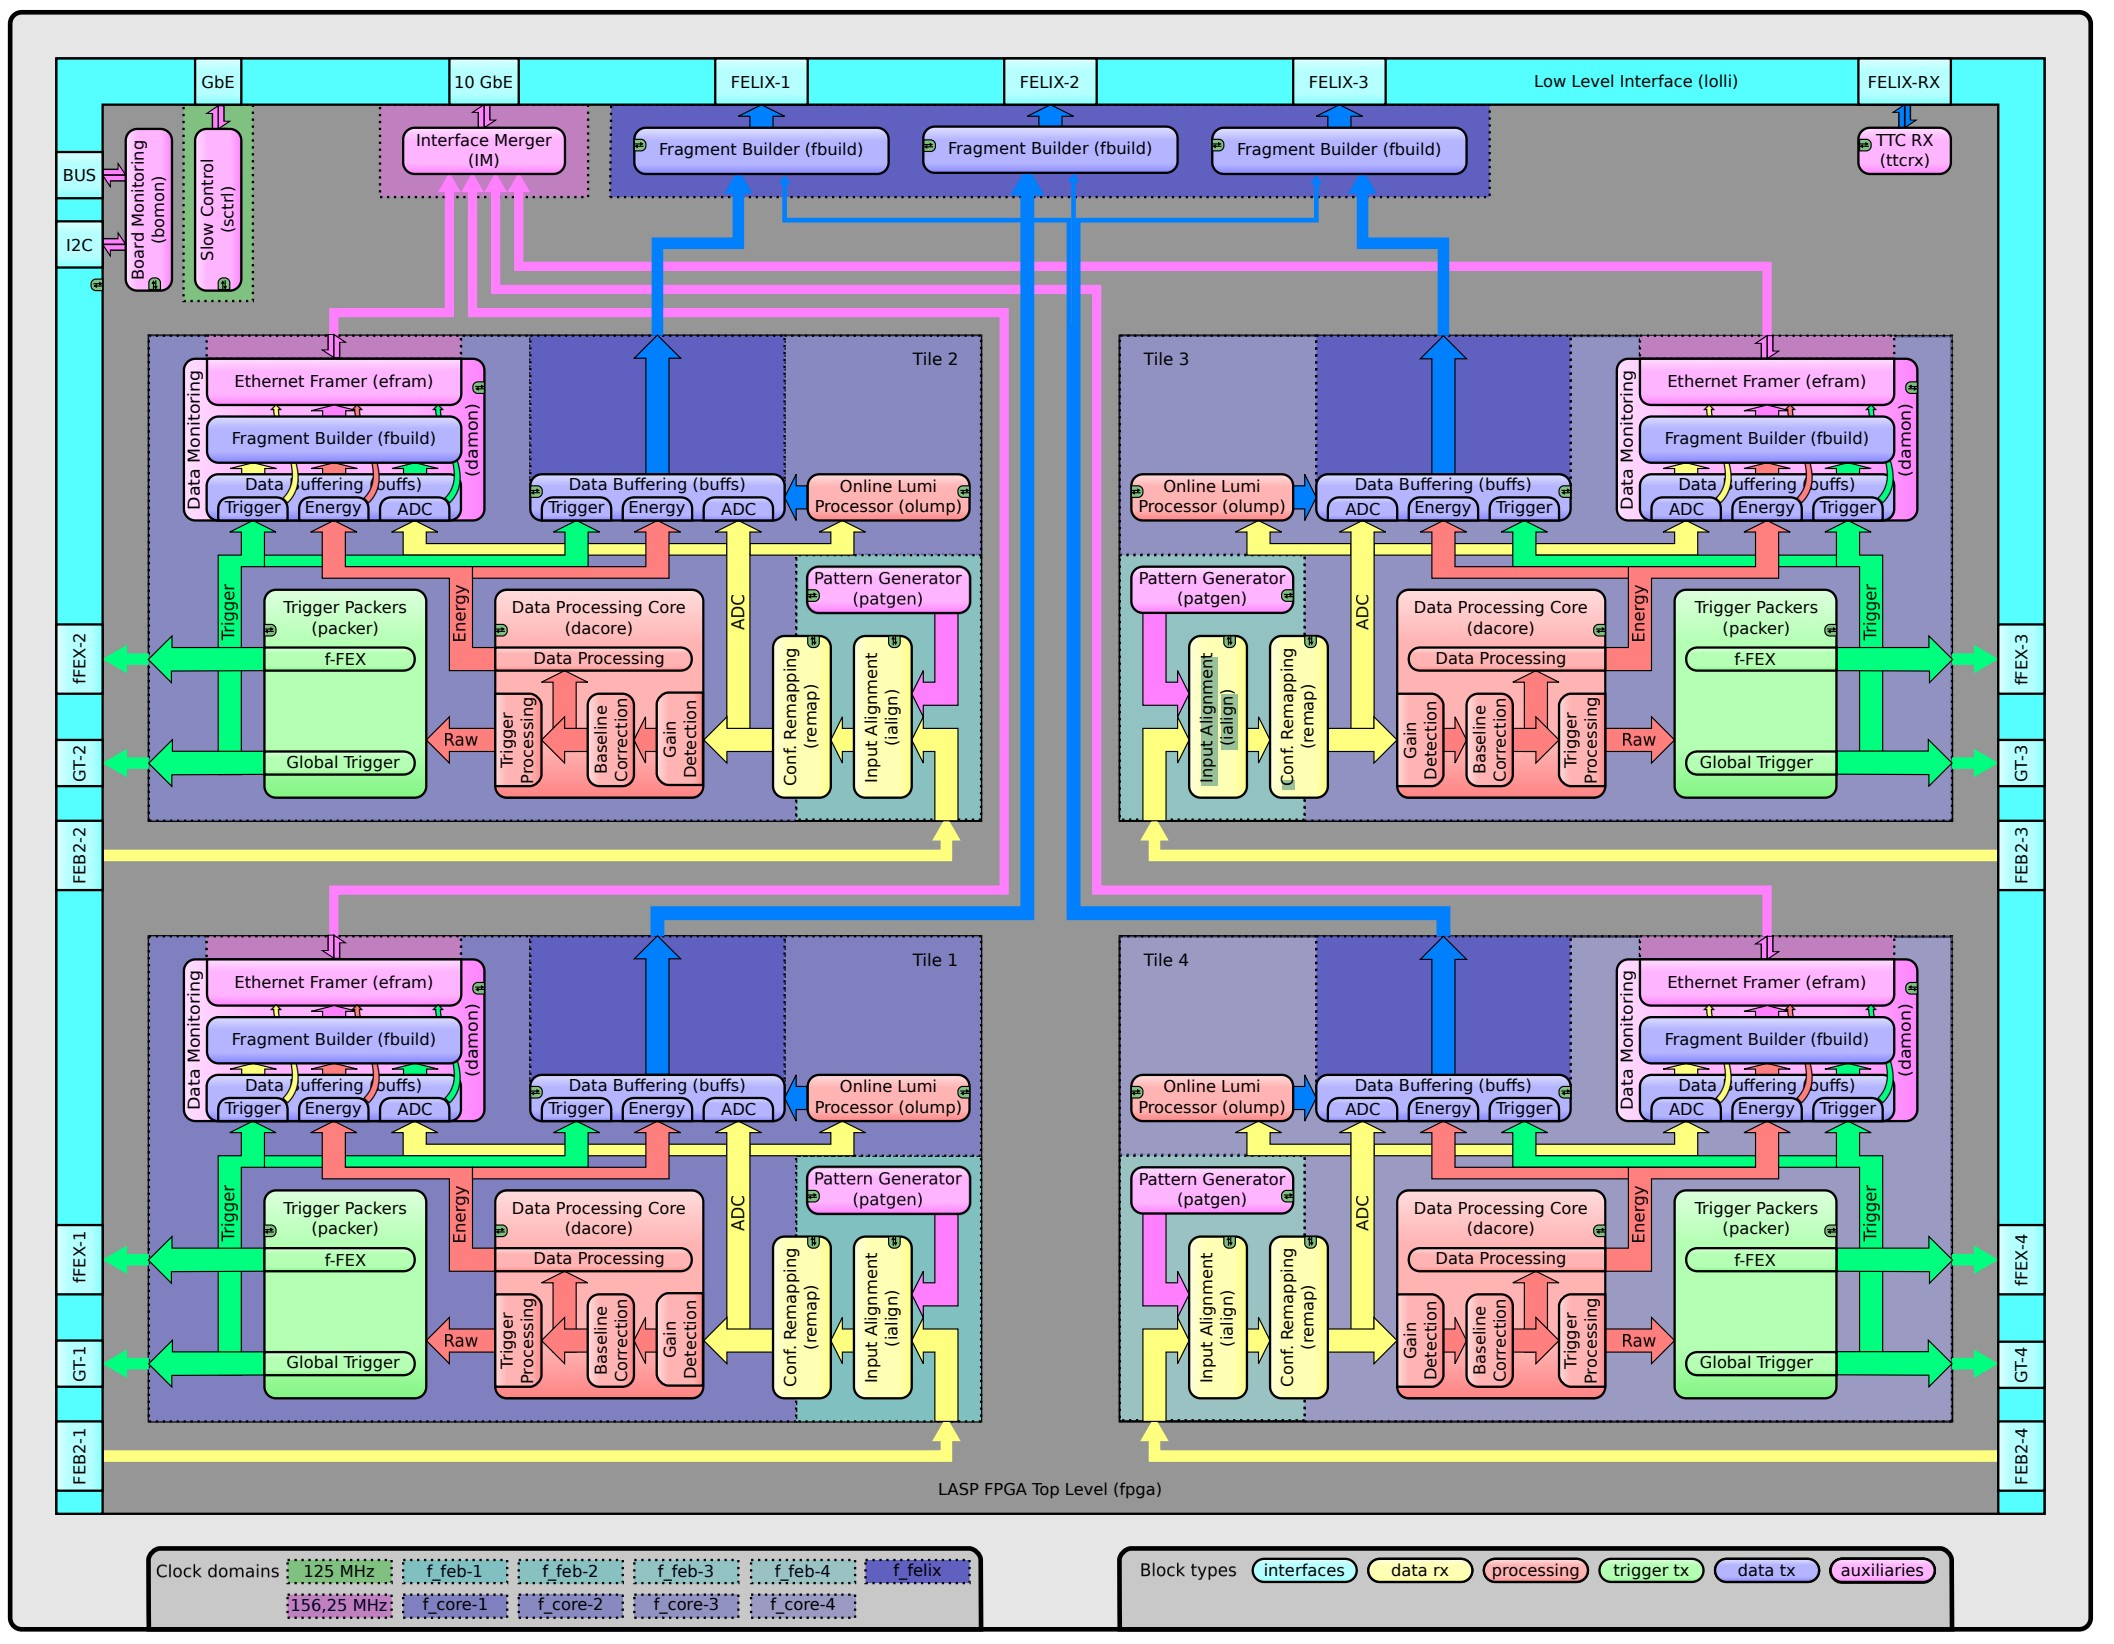
\includegraphics[width=\linewidth]{lasp_full.png}
    \caption{Полная блок схема архитектуры сигнального процессора LASP}
    \label{fig:lasp_full}
\end{figure}\par


